\chapter{基于时空分离策略的Non-Local时空图卷积模块}
%ST-GCN LTD-GCN Full-gcn
在第\ref{chapter-5}章中提到,设计合理的网络架构和学习策略,进而减少预测过程中的不确定性,是提高人体运动姿态预测精度的一个有效方法。但更多的方法,着眼于提升网络特征提取能力,通过从输入数据中获得更多的信息来降低预测过程中的不确定性。早期的方法借助循环神经网络在处理序列化数据上的优势,设计了基于RNN的人体运动姿态运动预测算法。但这类方法只考虑了数据的序列化特性,忽略了对重要的人体空间结构信息进行建模。随后的方法,注意到了图卷积网络在对不规则数据进行结构建模的能力。设计了使用GCN对人体结构信息进行建模的方法。但由于人体运动姿态数据包含时间和空间两部分,使用传统的图卷积网络进行建模时,邻接矩阵的规模将随着时空维度倍数增加。因此,有部分方法提出将时空信息的处理步骤分离,空间维度由GCN处理,时间维度则由TCN\cite{oord2016wavenet}处理。但TCN的卷积核大小限制了其感受野范围,不利于捕捉时间序列中长时依赖。鉴于现有方法存在的种种不足,我们提出了一种基于时空分离策略的Non-Local时空图卷积模块。该方法通过分离时空维度降低了网络的时间复杂度。在时间和空间维度均使用Non-Local的GCN算子,赋予网络全局感知能力。接下来,我们将首先介绍现有时空图卷积模块和本方案的设计思路以及优劣对比,随后再详细叙述基于时空分离策略的Non-Local时空图卷积模块的构造细节。

\section{时空图卷积模块设计思路对比}
再展示各个时空图卷积模块设计思路之前,我们首先展示人体运动姿态数据的时空结构特点。

\begin{figure}[ht]
    \centering
    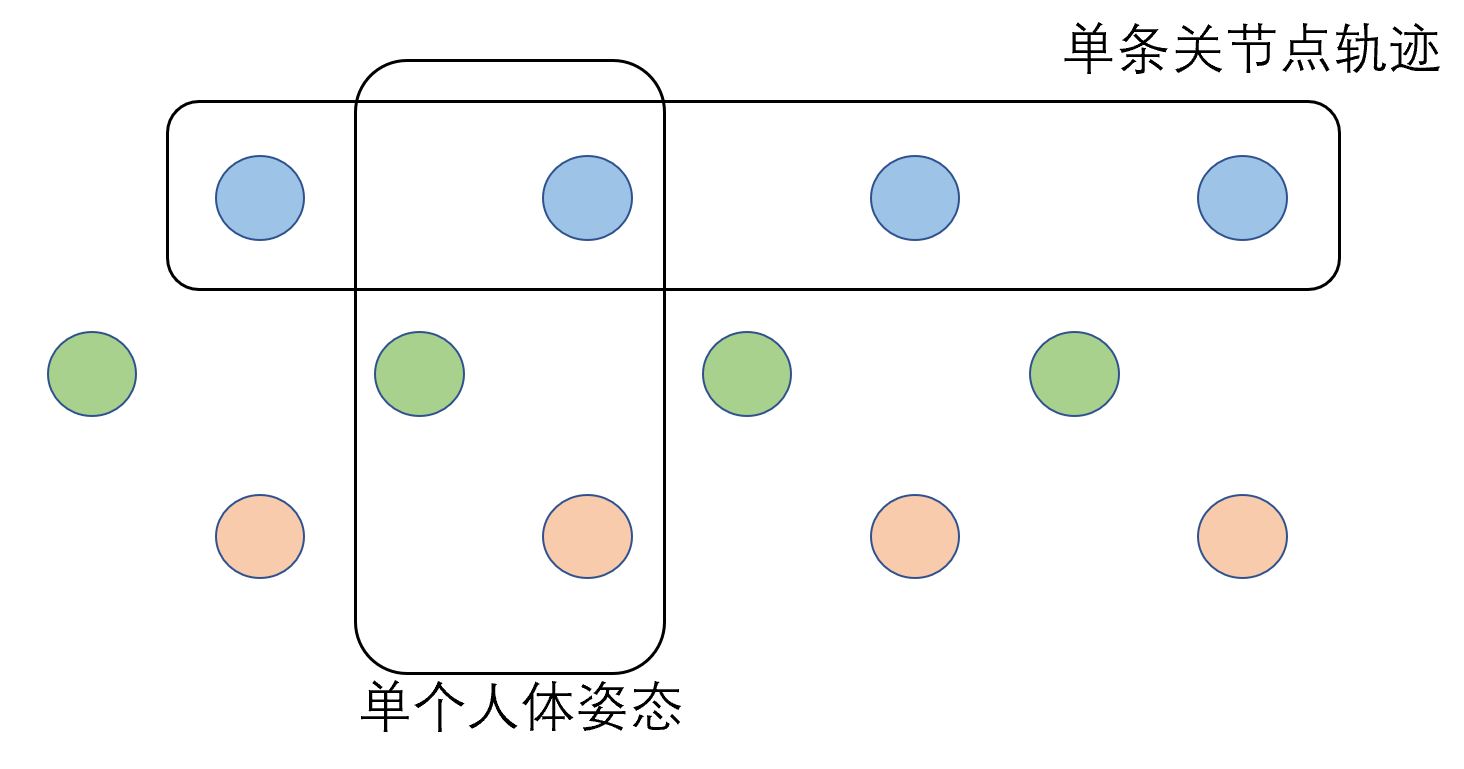
\includegraphics[width=0.80\textwidth]{FigMa/human_pose_seq.png}\\
    \vspace{-0.3cm}
    \caption{人体运动姿态数据时空结构}
    \label{fig:human_pose_seq_structure}
\end{figure}

如图\ref{fig:human_pose_seq_structure}所示,图中的彩色节点代表关节点,同一种颜色的节点代表某个关节点在时序上的运动轨迹(Trajectory)。同一时间点所有不同颜色的节点构成一个人体姿态。
在数学上,我们将上述人体运动姿态序列定义为一个时空无向图(spatialtemporal graph) $\mathcal{G} = \{\mathcal{V,E}\}$。其中,$\mathcal{V}$是对应人体运动姿态序列中所有关节点的节点集合。而$\mathcal{E}$是描述这些关节点对间联系的边集合。图\ref{fig:human_pose_seq_structure}展示了一个长度为4(T=4),每个姿态包含3个关节点(V=3)的人体运动序列。而时空图卷积模块的任务就是借助邻接矩阵$\mathbf{A}^{ST} \in \mathbb{R}^{VT\times VT}$对包含时间和空间两个维度的人体运动姿态序列进行建模。通过如下递归的时空图卷积网络可以提取到运动序列中的高阶语义信息。
\begin{equation}
    \mathbf{H}^{(l+1)}= \mathbf{A}_{ST}^{(l)}\mathbf{H}^{(l)}\mathbf{W}^{(l)},
    \label{equation:graph-conv}
\end{equation}
其中,$l$指第$l$时空图卷积层,$\mathbf{A}_{ST}^{(l)}\in \mathbb{R}^{VT\times VT}$则是该层描述时空依赖关系的邻接矩阵。$\mathbf{H}^{(l)}\in \mathbb{R}^{VT\times F^l}$是该层待处理的特征图,特征空间等于时空维度。$\mathbf{W}^{(l)}\in \mathbb{R}^{F^l\times F^{l+1}}$是特征映射权值矩阵,负责将关节点特征在特征空间上进行变换。最终,$\mathbf{H}^{(l+1)}$作为$\mathbb{R}^{VT\times F^{l+1}}$空间中的特征图被送往下一个阶段进行进一步处理。

在处理过程中,由于数据包含时间和空间两个维度,每个维度上的数据增加都会导致节点数量成倍膨胀,因此要求时空图卷积模块具有高效率。同时,为了对连续的时序数据和不规则的空间结构进行建模,时空图卷积模块需要具备较强的时空信息提取能力。而现有方法很难同时兼顾着两点要求。

\begin{figure}[ht]
    \centering
    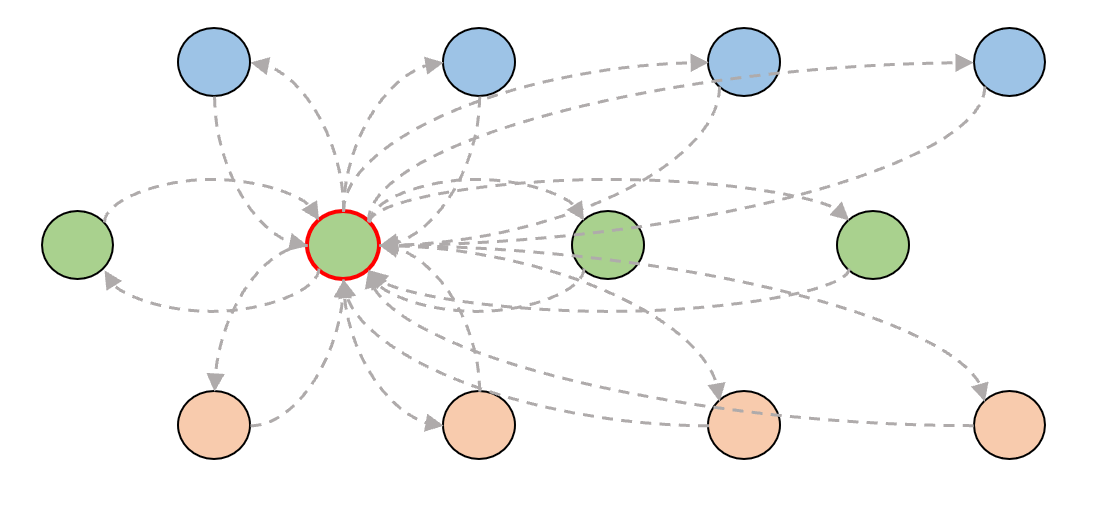
\includegraphics[width=0.80\textwidth]{FigMa/original_gcn.png}\\
    \vspace{-0.3cm}
    \caption{使用GCN同时对时空维度建模}
    \label{fig:original_gcn_structure}
\end{figure}

最直接的思路是如图\ref{fig:original_gcn_structure}所示使用一个GCN同时对时空两个维度进行建模,图中的虚线表示由邻接矩阵描述的关节点对间关系,图中红圈关节点的邻接关系规模为$\mathbb{R}^{VT}$。虽然该GCN可以通过邻接矩阵学习,不同空间位置、不同时间点的关节点对的联系。但这意味着在时空卷积层中,邻接矩阵的规模与数据时空维度相关$\mathbf{A}^{ST} \in \mathbb{R}^{VT\times VT}$,这将导致模型规模剧烈膨胀,严重降低模型的运行效率。同时,如此规模的网络也使得训练过程更加困难,容易出现欠拟合现象。因此该这设计并没有被实际应用。

\begin{figure}[ht]
    \centering
    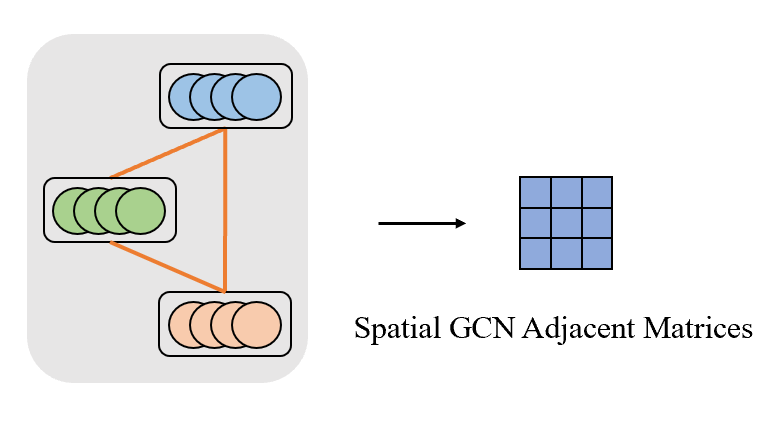
\includegraphics[width=0.8\textwidth]{FigMa/LTD_gcn.png}\\
    \vspace{-0.3cm}
    \caption{LTD中的图卷积模块}
    \label{fig:LTD_gcn_structure}
\end{figure}

作为率先使用GCN的方法,LTD提出:忽略在时序空间上对输入数据的时序结构进行建模,而是将关节点运动序列看作图卷积网络中的节点值,在特征空间上通过权值矩阵$W$对齐进行变换。具体GCN结构由图\ref{fig:LTD_gcn_structure}可见,其中由多个圆形组成的序列代表关节点运动序列,而它们被当作节点放入无向图中。该设计中,由于将关节点运动序列看作节点值$\mathcal{V}_S = \{v | v \in \mathbb{R}^{T} \}$,时序数据被组织为一个节点值为关节点运动序列的空间无向图。避免了对时间节点间的邻接关系进行建模,因此如公式\ref{equation:LTD}所示,只需要一个空间上的GCN对人体空间结构进行处理,大大降低模型的空间复杂度。
\begin{equation}
    \mathbf{H}^{(l+1)}= \mathbf{A}_{S}^{(l)}\mathbf{H}^{(l)}\mathbf{W}^{(l)},
    \label{equation:LTD}
\end{equation}
然而,该方法仅仅对人体空间结构进行建模,忽略了数据时序上的联系,时空信息提取能力并不完备,制约了模型对输入信息的提取与利用。

\begin{figure}[ht]
    \centering
    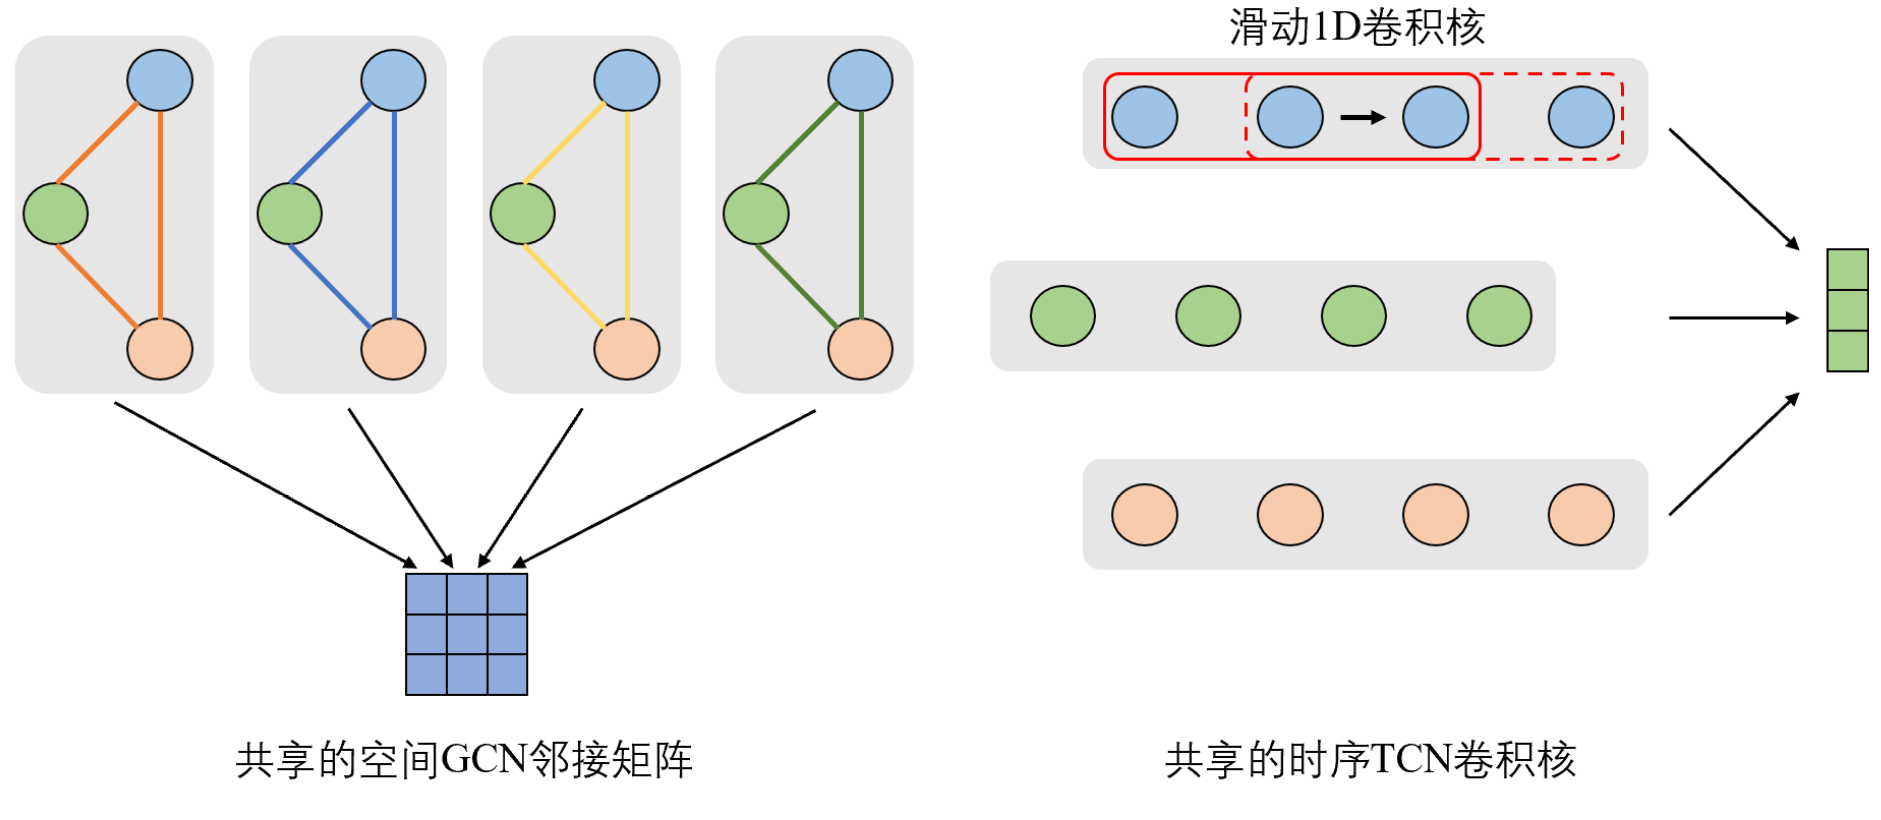
\includegraphics[width=1\textwidth]{FigMa/ST-GCN.png}\\
    \vspace{-0.3cm}
    \caption{ST-GCN中的图卷积模块}
    \label{fig:ST-GCN_structure}
\end{figure}
和LTD同期的工作ST-GCN\cite{yan2018spatial}提出了不同的思路,它使用了分离输入数据时间维度和空间维度的策略,分别设计算子对时间和空间信息进行提取。如图\ref{fig:ST-GCN_structure}所示。图左部分,为空间维度特征提取步骤,ST-GCN根据人体空间结构特征使用GCN进行建模,且通过参数共享机制降低模型的参数量,同一个运动序列,位于不同时间点的人体姿态共享一个图卷积网络,因为人体空间结构先验信息是普适通用的,不会随着时间位置的不同而变化,因此对位于不同时刻的人体姿态,可以使用同一个GCN处理。图右展示了时间维度特征提取步骤,不同于人体空间结构属于不规则无向图,时序上的关节点轨迹可以看作一条1D的规则数据,因此可以使用适用于1D结构数据建模的TCN\cite{oord2016wavenet}算子,TCN是一种继承自CNN的模型,其空间不变性特点得以保留。在进行空间特征提取时,TCN采用了参数共享的思路,以便将不同空间位置的关节点运动轨迹共享一个TCN。与CNN类似,TCN的卷积核也沿时间维度滑动,以提取时间信息。然而,这种设计导致模型在时间维度上的感受野受限于卷积核的尺度,从而限制了其长时依赖捕捉能力。综上,其卷积模块以公式\ref{equation:ST-GCN}形式表示,输入数据在经过GCN提取空间信息后,再由TCN提取时间信息,最终间接地捕捉到了数据中的时空信息。虽然ST-GCN较LTD,补全了模型在时序信息提取能力上的缺陷,但受限于感受野的局部性,在长时依赖捕捉能力上任然有所欠缺。
\begin{equation}
    \mathbf{H}^{(l+1)}= TCN(\mathbf{A}_{s}^{(l)}\mathbf{H}^{(l)}\mathbf{W}^{(l)}),
    \label{equation:ST-GCN}
\end{equation}

\begin{figure}[ht]
    \centering
    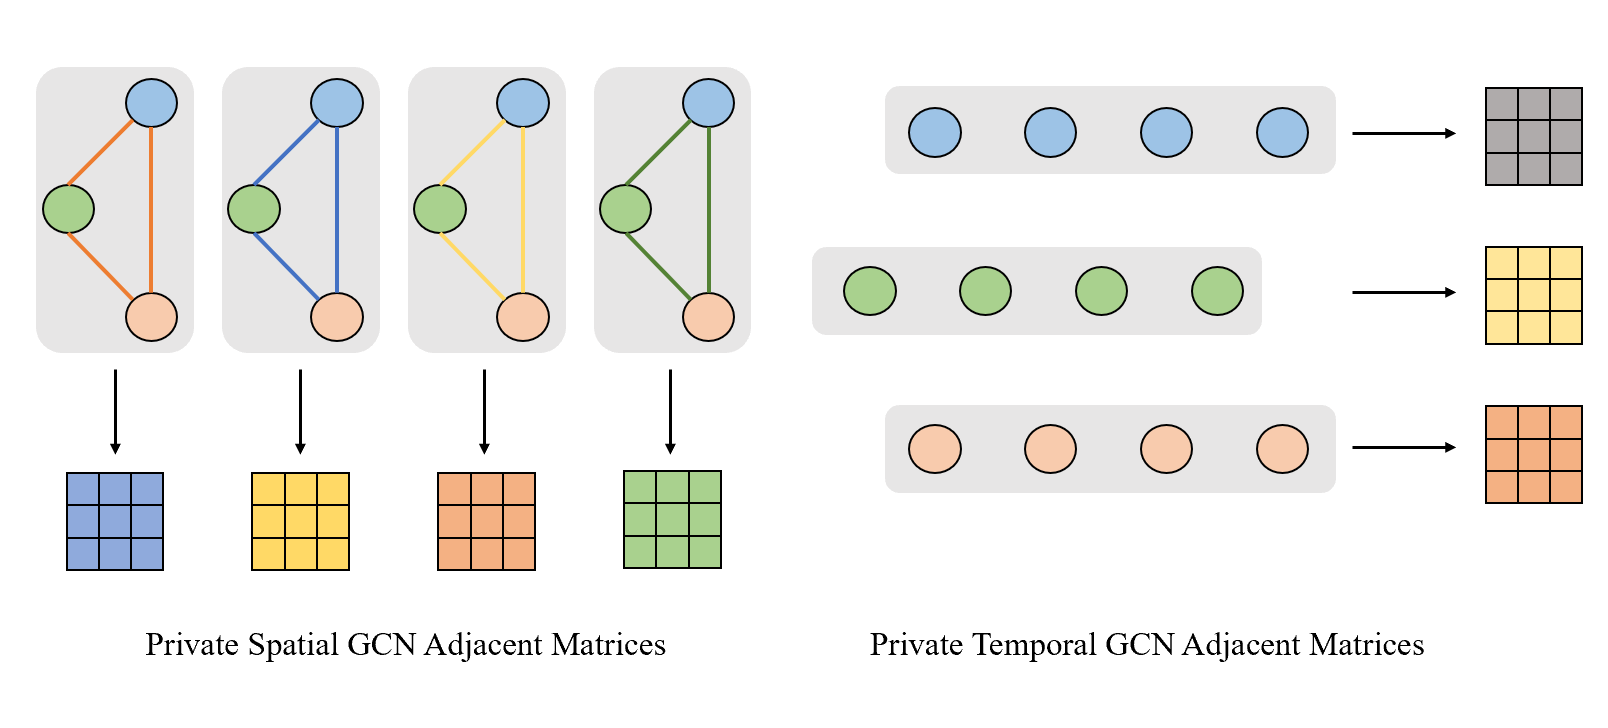
\includegraphics[width=1\textwidth]{FigMa/STS-GCN.png}\\
    \vspace{-0.3cm}
    \caption{STS-GCN中的图卷积模块}
    \label{fig:STS-GCN_structure}
\end{figure}

近来,STS-GCN\cite{sofianos2021space}提出了一种在时空维度均使用图卷积网络的方法,它扩展了图卷积网络(GCN)并添加了捕捉时间序列上人体姿势演变的时间卷积。与ST-GCN类似,它同样将时间和空间维度拆分。在空间维度上,它使用传统的图卷积网络对人体结构信息进行建模。在时间维度,与ST-GCN将关节点运动序列看作规则的1D数据不同,它选择用图结构来定义时序上关节点对的连接关系。具体的,它将关节点运动序列也视作一个无向不规则的图结构,图中的关节点不光被允许与邻接节点产生联系,还可以和序列中任意一个关节点建立邻接关系。这使得网络拥有了全局的时序信息感知能力,能捕捉更长时间范围内的运动信息。这将有助于网络从整体上理解输入运动序列,从而对未来运动序列做出更准确的预测。然而,与ST-GCN中同一时间维度或空间维度中的数据共享同一个特征提取模块不同,STS-GCN为不同时刻的人体姿态和不同空间位置的关节点运动轨迹设计了私有的特征提取模块。如图\ref{fig:STS-GCN_structure}中所示。对于不同时刻的人体姿态,STS-GCN为每一个都分配了一个不共享的空间图卷积。对于不同空间位置的关节点序列,则由对应的、私有的时间图卷积提取特征。这虽然在一定程度上提高了网络的冗余度。但由于不同的人体姿态和关节点轨迹在空间或时间上都具有相同的空间结构或时序位置,它们对网络来说是平等的,这种平等性的存在使得网络可以更加普适地处理不同的人体姿态和关节点轨迹,而无需为每种情况设计特定的特征提取模块。

\begin{figure}[ht]
    \centering
    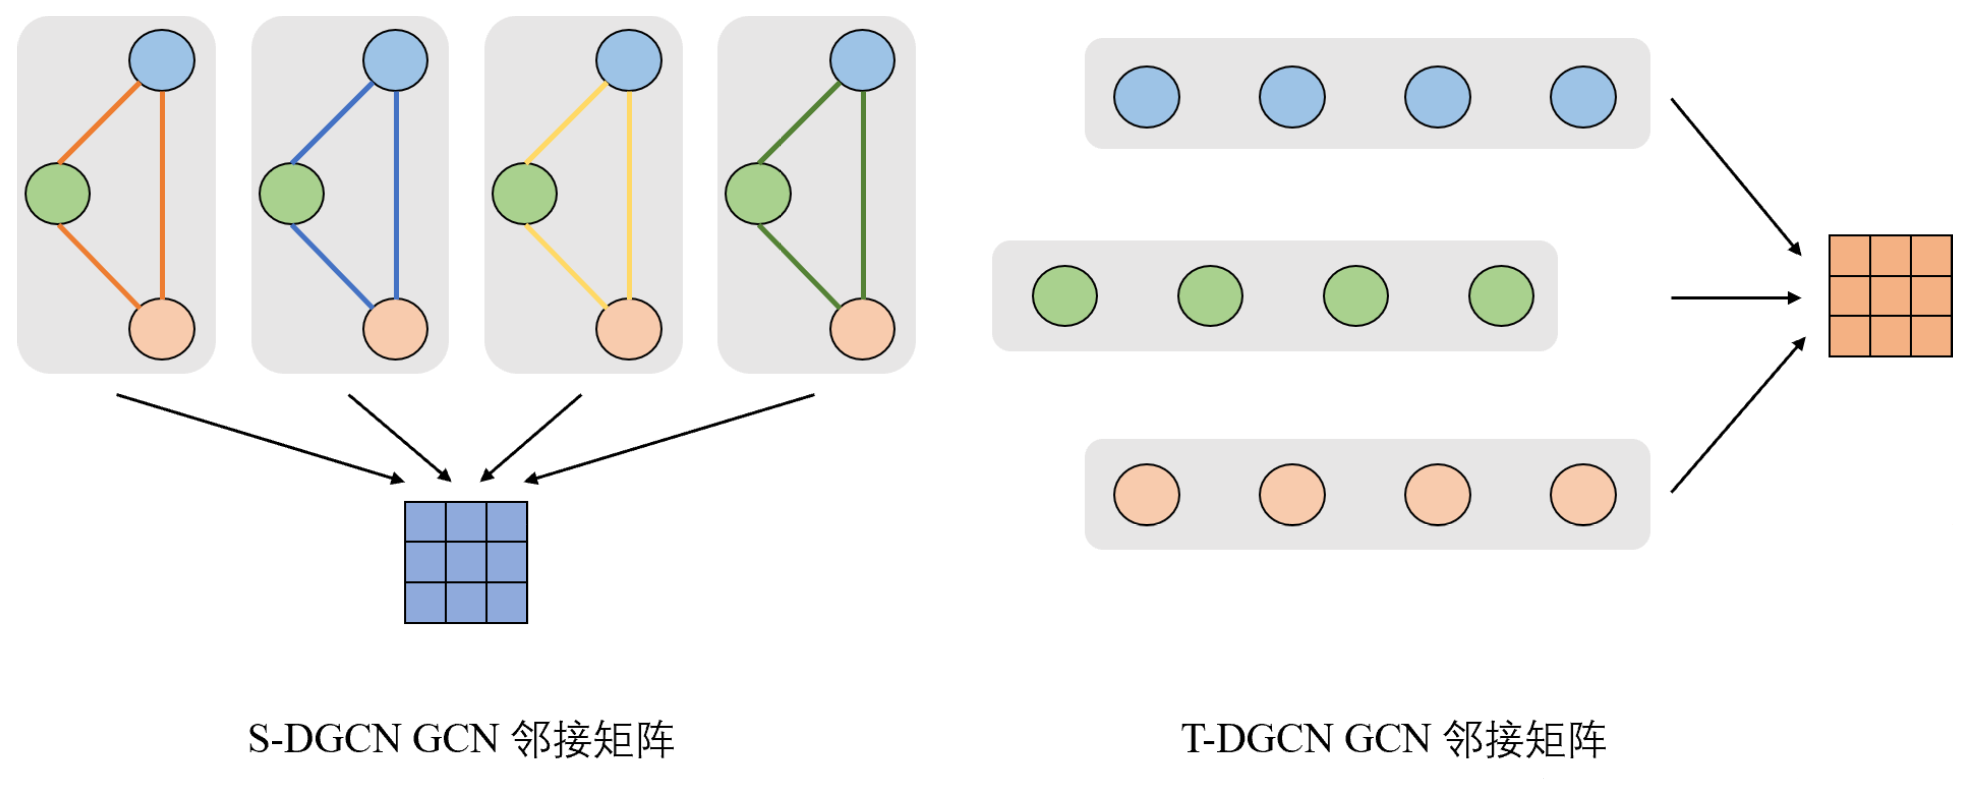
\includegraphics[width=1\textwidth]{FigMa/Our_gcn.png}\\
    \vspace{-0.3cm}
    \caption{基于时空分离策略的Non-Local时空图卷积模块}
    \label{fig:Our_gcn_structure}
\end{figure}
我们则基于对以上方法的分析提出了一种基于时空分离策略的Non-Local时空图卷积模块。如图\ref{fig:Our_gcn_structure}所示,首先,我们将数据的时空处理步骤进行解耦。分别分配S-DGCN(Spatial Dense GCN)和T-DGCN(Temporal Dense GCN)用于提取空间信息和时序信息,二者均为标准的GCN,可以捕捉时域和空域中的全局依赖,因此具有Non-Local的特性。值得注意的是,我们称二者为稠密(Dense)的GCN,因此部分现有方法\parencite{cui2020learning}中的邻接矩阵是以人为设计的方式定义,该类方法仅仅允许物理上有联系的关节点间建立联系,导致最终的邻接矩阵是稀疏的,只能处理低阶的连接关系。而真实环境中的由人体运动产生的关节互动是十分复杂的,例如,即使手肘与膝盖部位关节点没有物理上的连接,但在行走动作中,二者仍然会产生规律性的联系。我们认为人为地固定邻接矩阵将会削弱网络对高阶联系的捕捉能力。因此,我们将邻接矩阵设置为完全可学习的网络参数,赋予网络更高的灵活性。由网络根据训练数据自行定义关节点对间的邻接关系。为了降低网络规模,我们也使用了上文中提到的参数共享策略,同一个时空维度下的数据共享一个GCN。

\section{基于ST-DGCN的多阶段网络结构}
具体的,在实际网络中,假设第$l$层的特征图为$\mathbf{H}^{(l)}\in \mathbb{R}^{T\times V \times F^l}$,其中$F^l$指该层人体关节点特征维度的大小。我们通过公式\ref{equation:ST-DGCN}中的步骤更新特征图$\mathbf{H}^{(l)}$。首先数据经过S-DGCN提取空间信息,随后得到的中间结果被送入T-DGCN提取时间信息并输出到下一层。S-DGCN和T-DGCN以串联的形式结合。
\begin{equation}
    \begin{aligned}
        & {\widetilde{H}^{(l)}} = \text{S-DGCN}(H^{(l)}) = A^s H^{(l)} W^s, \text{(1)}
        \\
        & H^{(l+1)} = \text{T-DGCN}{\widetilde{H}^{(l)}} = A^t {\widetilde{H}^{(l)}} W^t, \text{(2)}
    \end{aligned}
    \label{equation:ST-DGCN}
\end{equation}

将公式\ref{equation:ST-DGCN}两个公式合并后,即可得到ST-DGCN(Spatial-temporal-DGCN)的表达式,其中$\mathcal{T}$代表对输入特征图的维度顺序进行交换,以使其满足矩阵相乘的维度要求,例如,提供一个$\mathbb{R}^{T\times V\times F^{l}}$的特征矩阵,$\mathcal{T}$维度变换操作,将其前两个维度顺序交换,最终输出的矩阵为$\mathbb{R}^{V\times T\times F^{l}}$。注意,$\mathcal{T}$仅仅改变维度顺序,不改变具体数据,这使得$\mathcal{T}$是一个可逆操作。
\begin{equation}
    \mathbf{H}^{(l+1)} = \mathcal{T}\left(
    \mathbf{A}_{t}^{(l)}t
    \left(
    \mathcal{T}
    \left(
    \mathbf{A}_{s}^{(l)}\mathbf{H}^{(l)}\mathbf{W}_s^{(l)}
    \right)
    \right)
    \mathbf{W}_t^{(l)}
    \right),
    \label{equation:ST-DGCN_ensemble}
\end{equation}

\begin{figure}[ht]
    \centering
    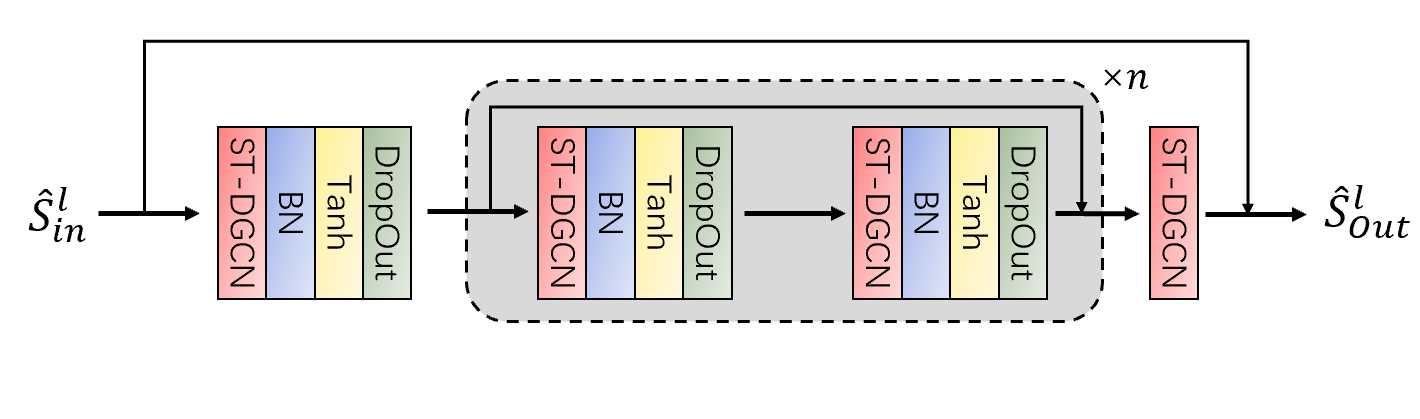
\includegraphics[width=1\textwidth]{FigMa/stage_network.png}
    \vspace{-0.3cm}
    \caption{基于ST-DGCN的单阶段网络结构}
    \label{fig:stage_network_structure}
\end{figure}

图\ref{fig:stage_network_structure}展示了单个阶段的详细网络结构,对应多阶段网络模型中的每个子阶段(Stage)。在第\label{chapter-5}章中曾提到,我们所设计的多阶段网络具有较灵活的通用性。具体的,多阶段网络框架中的特征提取模块可以根据具体任务灵活更换,做到即插即用,与网络框架解耦。因此,在将ST-DGCN应用到图\ref{fig:multi-stage}中时,不需要对网络结构做出过多修改,只需要用ST-DGCN替换网络中的原始GCN。特征提取模块中的最基本构成部分为GCL(Graph Convolution Layer),由ST-DGCN、Batchnorm、Tanh、DropOut构成。其中ST-DGCN又包含一对串联的S-DGCN、T-DGCN。两个GCL构成一个GCB(Graph Convolution Block),一个局部的残差连接跨越整个GCB,如图中的灰色矩形部分所示。每个阶段包含$n$个GCB。为了控制参数规模,整个网络包含的GCB数量固定不变,若阶段数量增多,则每个阶段包含GCB数量下降,我们将在实验部分探讨最佳的阶段数。最后,一个大的残差连接建立在该网络的输入与输出之间,被用来提高训练效率,对结果施加一致性约束。

在训练模式下,输入数据$\hat{S}^l_in$首先经过一个位于网络入口处的GCL,它对输入特征的特征空间进行映射,保证与后续网络隐空间维度一致。后续的$n$个GCB对输入特征进行进一步的特征提取。最后得到的特征经过一个ST-DGCN映射后得到该阶段的预测结果。注意,最后一部分由一个独立的ST-DGCN构成,不包含额外的Batchnorm、Tanh和DropOut。因为该部分需要输出直接的结果,不应对特征施加额外的修改。随后该输出结果接受中级监督目标的约束(如果该阶段是最后一个阶段则直接接受真值的约束。)并传递给下一阶段。最终,将\ref{fig:stage_network_structure}中所述网络复制多次,以串联的形式连接,最终即可得到图\ref{fig:multi_stage}中的多阶段网络。

\section{总结}
在本章节中,我们介绍了基于时空分离策略的Non-Local时空图卷积模块,称为ST-DGCN。首先,我们从具有代表性的现有方法入手,分析了当前几种被广泛使用的具有时空信息提取能力的图卷积模块。经过详细调研,我们发现现有方法在时序数据处理能力、网络效率、长时依赖捕捉能力方面有所欠缺。具体的,LTD\cite[mao2019learning]选择牺牲网络的时间依赖提取能力,换来网络效率的提升。它放弃直接对时序信息建模,将关节点运动轨迹视作一个整体,在特征空间中对其进行变换。因此可以使用传统的GCN仅仅对空间接口进行建模,将网络时间复杂度控制在较低的水平。同期的工作,ST-GCN\cite{yan2018spatial}则使用轻量化的TCN对时序数据进行建模,但受限于卷积核的大小,模型难以捕捉长时的时序依赖。STS-GCN更近一步,将GCN推广到了时间维度,建立一统一的时空GCN模型,但其设计存在冗余,时空效率不高。

在总结以上方法的优劣势后,我们提出了ST-DGCN,该模块的设计思路为:(1)通过时空分离的策略,将图卷积网络推广到时间和空间维度,以间接的方式建立一个高效的时空GCN模块,赋予网络Non-Local的特性。(2)通过人体姿态和关节点序列间的参数共享,控制网络参数规模,保证网络效率。最终我们实现了预测精度和时空效率的均衡,具体我们将在实验部分进一步讨论。另外,得益于第\ref{fig:multi_stage}章中,我们的多阶段模型的高度灵活性和拓展性,ST-DGCN可以轻易地应用于该多阶段模型中,我们将在随后的实验证明,ST-DGCN较强的时空信息提取能力将帮助提升网络的预测性能。